\documentclass{zapiski}

\originfo{529}{}{}{2026}
\setcounter{page}{1}
\date{}

\usepackage[cp1251]{inputenc}
\usepackage[T2A]{fontenc}
\usepackage[russian, english]{babel}

\usepackage{amsmath, amssymb, amsthm, mathtools, bm}

\usepackage{graphicx}
\usepackage{booktabs}
\usepackage{caption}
\usepackage{float}
\usepackage{enumitem}

\usepackage[unicode, colorlinks=true, linkcolor=blue, urlcolor=blue]{hyperref}

\usepackage{amsthm}

\theoremstyle{plain}
\newtheorem{theorem}{Theorem}[section]
\newtheorem{lemma}[theorem]{Lemma}

\theoremstyle{definition}
\newtheorem{definition}{Definition}[section]
\newtheorem{assumption}{Assumption}[section]

\theoremstyle{remark}
\newtheorem*{remark}{Remark}

\newcommand{\norm}[1]{\left\lVert #1 \right\rVert}
\DeclareMathOperator{\RMS}{RMS}
\DeclareMathOperator{\FFN}{FFN}
\DeclareMathOperator{\MSA}{MSA}
\DeclareMathOperator{\TB}{TB}
\DeclareMathOperator{\blockdiag}{blockdiag}


\begin{document}

\title[Jacobian Analysis of Transformers]{Jacobian Analysis of a Recurrent Transformer Block}

\author{
  \textbf{Dmitrii Vasilenko\textsuperscript{1}},
  \textbf{Ilia Stepanov\textsuperscript{1}},
  \textbf{Vadim Kasiuk\textsuperscript{1}},
  \textbf{Gleb Karpeev\textsuperscript{1}},
  \textbf{Andrey Grabovoy\textsuperscript{1,2}}
\\ \vspace{0.2cm}
  \textsuperscript{1}Moscow Institute of Physics and Technology\\
  \textsuperscript{2}V.A. Trapeznikov Institute of Control Sciences of Russian Academy of Sciences
\\ \vspace{0.2cm}
  {\small \textbf{Correspondence:} \href{mailto:vasilenko.dmitrii@phystech.edu}{vasilenko.dmitrii@phystech.edu}}
}

\begin{abstract}
Recurrent Transformers are a parameter-efficient approach for modeling deep computations, but their deployment in iterative settings requires controlled and stable dynamics. We study the Jacobian dynamics of a full Transformer block with Multi-Head Self-Attention (MSA), Feed-Forward Networks (FFN), and RMS normalization. We derive an explicit upper bound on the spectral norm of the full-step Jacobian, showing that RMSNorm acts as a multiplicative damping factor that prevents gradient explosion. Under mild assumptions, the Jacobian norm remains $O(1)$ in the large-step regime. Our theoretical results, validated on synthetic and CIFAR-10 data, provide insight into stability properties of recurrent models.
\end{abstract}

\keywords{Recurrent Transformers \and Jacobian dynamics \and RMS normalization \and Stability analysis \and Mechanistic interpretability.}

\maketitle


\section{Introduction}

Self-attention (SA) is the core mechanism of Transformer blocks~\cite{DBLP:journals/corr/VaswaniSPUJGKP17}. Recent theory has revealed behaviors of SA layers such as spectral phenomena, rank collapse~\cite{noci2022signalpropagationtransformerstheoretical}, and limits of expressive power~\cite{yun2019transformers,kajitsuka2023transformers,nichani2024understanding}. Understanding SA dynamics is thus central to explaining stability, generalization, and multi-step reasoning.

A common theoretical view interprets attention updates as energy-minimizing processes, where the monotone decrease of an energy function explains clustering and rank collapse~\cite{ramsauer2020hopfield,yang2022transformers,hoover2024energy,geshkovski2023mathematical,geshkovski2024emergence,geshkovski2024dynamic,bruno2025emergence}.  

An alternative, energy-agnostic approach uses the Jacobian of the recurrent update. Tomihari and Karakida~\cite{tomihari2025recurrentselfattentiondynamicsenergyagnostic} showed that RMSNorm stabilizes looped SA by suppressing the Jacobian spectral norm, ensuring stability even for large updates.

We extend this framework to a \textit{full Transformer block} including MSA, FFN, residuals, and normalization, and investigate whether stability guarantees hold in this realistic setting.

Analyzing a full Transformer block is non-trivial compared to previous studies of standalone self-attention. The integration of Feed-Forward Networks (FFN) and interleaved residual connections creates compounded dynamics where the damping effect of RMSNorm must counteract the combined expansion of both MSA and FFN layers.

Our contributions are:
\begin{itemize}
    \item Row-wise RMSNorm stabilizes the full block under mild norm assumptions, damping amplification from both MSA and FFN.
    \item An explicit upper bound on the Jacobian spectral norm for the complete block.
    \item Theoretical stability guarantee: the Jacobian norm remains bounded ($O(1)$) even for large updates.
    \item Empirical validation on synthetic and CIFAR-10 embeddings confirms the bounds.
\end{itemize}


\section{Related Work}

\paragraph{Energy-based understanding.}
Many works model recurrent self-attention via energy functions~\cite{geshkovski2023mathematical,geshkovski2024emergence,geshkovski2024dynamic,bruno2025emergence,karagodin2024clustering}, explaining clustering and rank collapse. Other studies~\cite{yang2022transformers,ramsauer2020hopfield,hoover2024energy} cast attention as energy-minimizing, but often rely on simplifications (e.g., single-head attention, symmetric weights), limiting applicability to standard Transformers.

\paragraph{Jacobian-based analysis.}
Jacobian analysis is a classical tool to study stability of neural systems~\cite{boedecker2012information,poole2016exponential,pennington2017resurrecting,haber2017stable,chang2019antisymmetricrnn,yoshida2017spectral,lewandowski2024learning}. For attention, prior work analyzed Jacobian spectra to explain rank collapse~\cite{noci2022signalpropagationtransformerstheoretical,castin2023smooth}. Closest to ours is Tomihari and Karakida~\cite{tomihari2025recurrentselfattentiondynamicsenergyagnostic}, who provided an energy-agnostic Jacobian analysis for a recurrent SA block. We extend this to a full Transformer block including FFN.

\paragraph{Looped architectures.}
Looped Transformers reuse block parameters across iterations, decoupling computational depth from model size and improving efficiency~\cite{dehghani2018universal}. Studies show they can learn algorithmic tasks and enhance reasoning biases~\cite{yang2023looped,giannou2023looped,saunshi2025reasoning}, and scale experiments explored iteration counts~\cite{geiping2025scaling,bansal2022end}. Related ideas include weight-tying~\cite{lan2019albert}, equilibrium models~\cite{bai2019deep}, and biologically inspired loops~\cite{miyato2024artificial}. We focus on realistic looped blocks with standard MSA, FFN, and RMSNorm, with rigorous Jacobian diagnostics.

\section{Methodology}
\label{sec:method}

In this section we give a self-contained formulation of the iterative Transformer block
as a discrete dynamical system, introduce all notation used throughout the paper, derive operator
derivatives used in the Jacobian analysis, and describe the numerical procedures and experimental
protocol used to validate the theoretical bounds.

\subsection{Notation and preliminaries}
\label{ssec:notation}

Let $S$ denote sequence length and $D$ denote the hidden dimension. We write the state at
discrete time (iteration) $t$ as $ Y^{(t)} \in \mathbb{R}^{S\times D}.$

For a matrix $A$ we denote by $A[i,j]$ the $(i,j)$-entry, by $A[i,:]\in\mathbb{R}^D$ the $i$-th row
(token vector) and by $A[:,j]\in\mathbb{R}^S$ the $j$-th column. For a vector $x\in\mathbb{R}^D$
we use the Euclidean norm $\|x\|_2$, for a matrix $B$ we use the operator (spectral) norm
$\|B\|_2$. All Jacobians are given in \emph{numerator-layout}, e.g. for a function
$f:\mathbb{R}^D\to\mathbb{R}^D$ we write
\[
J_f(x) \;=\; \frac{\partial f(x)}{\partial x} \in \mathbb{R}^{D\times D}.
\]
Jacobians with respect to the full state $Y\in\mathbb{R}^{S\times D}$ are interpreted as
block Jacobians of size $(SD)\times (SD)$.

\subsection{Basic building blocks}
\label{ssec:blocks}

Below we define the concrete algebraic form of the modules used inside the iterative block:
multi-head self-attention, position-wise feed-forward network and RMS normalization.

\paragraph{Multi-head self-attention (MSA).}
\label{sssec:msa}

Let $H$ be the number of attention heads and $d_h = D/H$ the per-head dimension. For a state
$Y\in\mathbb{R}^{S\times D}$ define the linear projections
\begin{align}
Q &= Y W_Q,\qquad K = Y W_K,\qquad V = Y W_V, \label{eq:proj}
\end{align}
where $W_Q,W_K,W_V\in\mathbb{R}^{D\times D}$ are learned matrices. We split $Q,K,V$ into heads
by contiguous blocks: for $h=1,\dots,H$ let $Q_h\in\mathbb{R}^{S\times d_h}$ denote the columns
$(h-1)d_h{:}hd_h$ of $Q$, and likewise for $K_h,V_h$. The attention weights for head $h$ are
\begin{align}
A_h &= \operatorname{softmax}\!\Big(\frac{Q_h K_h^\top}{\sqrt{d_h}}\Big)\in\mathbb{R}^{S\times S},
\end{align}
(the softmax is applied row-wise). The head output is $Z_h = A_h V_h\in\mathbb{R}^{S\times d_h}$.
Concatenating heads and applying an output projection $W_O\in\mathbb{R}^{D\times D}$ yields

\begin{equation}
\begin{gathered}
\operatorname{MSA}(Y) = Z W_O, \\
Z=[Z_1\;\|\;Z_2\;\|\;\dots\;\|\;Z_H]\in\mathbb{R}^{S\times D}.
\end{gathered}
\end{equation}

\paragraph{Position-wise feed-forward network (FFN).}
\label{sssec:ffn}

The position-wise FFN is applied row-wise (token-wise):
\begin{align}
\operatorname{FFN}(Y) \;=\; \sigma( Y W_1 + \mathbf{1} b_1^\top ) W_2 + \mathbf{1} b_2^\top,
\end{align}
where $W_1\in\mathbb{R}^{D\times D_{ff}}$, $W_2\in\mathbb{R}^{D_{ff}\times D}$, $b_1\in\mathbb{R}^{D_{ff}}$,
$b_2\in\mathbb{R}^{D}$, $\mathbf{1}\in\mathbb{R}^{S\times 1}$ is a column of ones, and
$\sigma(\cdot)$ is a pointwise nonlinearity (e.g. GELU). All operations are applied independently to each row.

\paragraph{RMS normalization (RMSNorm).}
\label{sssec:rms}

We adopt the Root Mean Square Layer Normalization proposed by Zhang and Sennrich~\cite{zhang2019root}. We analyze an L2-based RMS normalization variant, which is equivalent to RMSNorm up to a constant scaling factor.

For a token vector $y\in\mathbb{R}^D$ and a learned scale vector $\gamma\in\mathbb{R}^D$ we define
\begin{align}
\operatorname{RMSNorm}(y) \;=\; \operatorname{diag}(\gamma)\, \frac{y}{\|y\|_2}.
\end{align}
Applied to a matrix $Y\in\mathbb{R}^{S\times D}$ this is done row-wise:
$\operatorname{RMSNorm}(Y)_{[i,:]} = \operatorname{RMSNorm}(Y_{[i,:]})$.

\subsection{Iterative Transformer block: discrete dynamics}
\label{ssec:itr_block}

We now define the iterative Transformer block as a discrete-time mapping $F:\mathbb{R}^{S\times D}\to\mathbb{R}^{S\times D}$ that will be repeatedly applied to the state. The internal structure of our block follows a standard design, consisting of a sequence of two sub-blocks (MSA and FFN). Each sub-block employs a residual connection followed by RMS normalization, a configuration commonly known as \textit{"Post-Norm"}. This is the architecture analyzed in our theoretical derivations.

Let $C\in\mathbb{R}^{S\times D}$ denote an external context (e.g., input embeddings). The internal sequence of operations is defined as follows.
First, the input $Y$ passes through the MSA sub-block to produce an intermediate state $Y'$:
\begin{align}
    Y' = \operatorname{RMSNorm}(Y + \operatorname{MSA}(Y)) \label{eq:subblock1_final}
\end{align}
Then, this intermediate state $Y'$ passes through the FFN sub-block to produce the final block output, $\operatorname{TB}(Y)$:
\begin{align}
    \operatorname{TB}(Y) = \operatorname{RMSNorm}(Y' + \operatorname{FFN}(Y')) \label{eq:subblock2_final}
\end{align}
Finally, the full per-step update of the recurrent system is defined as:
\begin{align}
    \Delta Y^{(t)} &= C + \operatorname{TB}\big(Y^{(t)}\big), \label{eq:deltaY_final}\\
    U\big(Y^{(t)}\big) &= Y^{(t)} + \nu\,\Delta Y^{(t)},\qquad \nu>0 \ \text{(step coefficient)},\\
    Y^{(t+1)} &= \operatorname{RMSNorm}\big(U(Y^{(t)})\big). \label{eq:update_final}
\end{align}
Hence the complete iteration mapping is given by:
\begin{equation}\label{eq:F_def_final}
    F(Y) \;=\; \operatorname{RMSNorm}\!\big(Y + \nu(C+\operatorname{TB}(Y))\big).
\end{equation}
We study the local stability of repeated application of $F$ by analyzing its Jacobian, $J_F(Y)=\partial F(Y)/\partial Y$.

\subsection{Analytic Jacobian upper bounds}
\label{ssec:analytic}

This subsection develops explicit upper bounds on the operator norm $\|J_F(Y)\|_2$
 . The bounds  show that — under mild assumptions on the normalization inputs — the Jacobian operator norm remains uniformly bounded even in the large step-size regime.



\subsubsection{Composed bound for the full block}
\label{sssec:composed_bound}

This theorem generalizes the bound derived for MSA-only blocks in~\cite{tomihari2025recurrentselfattentiondynamicsenergyagnostic}. Our result explicitly incorporates the influence of the feed-forward network (via $\|J_{\FFN}\|$) and the inner normalization layers of a complete "Post-Norm" Transformer block.

\begin{theorem}\label{thm:jacobian_bound_final}
Let the iterative map $F(Y)$ be defined by Eqs.~\eqref{eq:subblock1_final}-\eqref{eq:update_final}. Suppose that the inputs to the three distinct RMSNorm layers in the update path satisfy the following lower bound conditions on their row-wise norms for all sequence indices $i$:
\begin{enumerate}[label=(\roman*)]
    \item $\norm{(Y + \operatorname{MSA}(Y))_{[i,:]}} \ge r_{in}$ (input to the first inner RMSNorm),
    \item $\norm{(Y' + \operatorname{FFN}(Y'))_{[i,:]}} \ge r_{out}$ (input to the second inner RMSNorm, where $Y'$ is defined in Eq.~\eqref{eq:subblock1_final}),
    \item $\norm{(Y + \nu(C+\operatorname{TB}(Y)))_{[i,:]}} \ge r_U$ (input to the final, outer RMSNorm).
\end{enumerate}
Let \(\gamma \in \mathbb{R}^D\) denote the learned scale vector in RMSNorm, and define 
\(\gamma_{\max} = \max_j |\gamma_j|\).  

Then the spectral norm of the Jacobian satisfies:

\begin{align}
    \|J_F(Y)\|_2 \le 
    \frac{\gamma_{\max}}{r_U}
    \Bigg( 
        1 + 
        \nu \frac{\gamma_{\max}^2}{r_{out} r_{in}}
        \times \left(1 + \|J_{\FFN}\|\right) \left(1 + \|J_{\MSA}\|\right)
    \Bigg),
\end{align}

where $\|J_{\FFN}\|$ and $\|J_{\MSA}\|$ are the spectral norms of the Jacobians of the FFN and MSA blocks respectively.
\end{theorem}

See Appendix~\ref{app:jacobian-proof} for the proof of Theorem~\ref{thm:jacobian_bound_final}.

We should note that such lower bounds are empirically satisfied after a small number of iterations and are consistent with mild assumptions and training regimes (see Section~\ref{ssec:exp_bounds}).


\subsubsection{Asymptotic compensation for large step-size $\nu$}
\label{sssec:asymptotics}

\begin{theorem}
\label{thm:JF_asympt}
Under the assumptions of \textbf{Theorem 3.1} and additionally assuming the non-degeneracy condition
\begin{equation}
\min_i \| \Delta Y_{[i,:]}\|_2 \ge \varepsilon > 0,
\end{equation}
the spectral norm of the Jacobian remains bounded as $\nu \to \infty$, i.e.,
\[
\|J_F(Y)\|_2 = O(1).
\]
\end{theorem}

\begin{remark}
The lower bound conditions $r_{in}, r_{out}, r_U > 0$ effectively prevent the vanishing of token representations. In our experiments, these row norms remain strictly positive and stable, as RMSNorm inherently projects inputs toward a fixed-norm hypersphere, preventing the collapse to the origin that would be required to violate these assumptions.
\end{remark}

See Appendix~\ref{app:JF_asympt} for the proof of Theorem~\ref{thm:JF_asympt}.

\section{Experimental Results}
\label{sec:results}

We now present the experimental validation of the theoretical Jacobian bounds derived in Section~\ref{sec:method}.
All experiments utilize the iterative Transformer block defined in Eq.~\eqref{eq:F_def_final}, configured with multi-head self-attention,
position-wise FFN with GELU activation, and row-wise RMS normalization.

\subsection{Validation of Theoretical Bounds}
\label{ssec:exp_bounds}

% First, we validate the upper bound on the spectral norm derived in Theorem~\ref{thm:jacobian_bound_final} using synthetic data.
% We vary the step coefficient $\nu \in [0.1, 2.0]$ for a typical model configuration ($S=32$, $D=64$, $H=4$, $D_{ff}=128$).
% For each $\nu$, we compute the empirical spectral norm $\|J_F(Y)\|_2$ via power iteration and compare it against the theoretical bound calculated using the measured component norms ($M=\|J_{\MSA}\|_2$, $F=\|J_{\FFN}\|_2$) and the minimal row norms ($r_U, r_{in}, r_{out}$).

First, we validate the upper bound derived in Theorem~\ref{thm:jacobian_bound_final}. The empirical spectral norm $\|J_F(Y)\|_2$ is estimated using the power iteration method applied to the Jacobian matrix. As shown in Figure~\ref{fig:full_spectral}, the empirical norm consistently stays below our theoretical estimate. While the derived bound is conservative due to the accumulation of worst-case estimates in the chain rule, it accurately tracks the growth pattern of the Jacobian as a function of the step size $\nu$, confirming its structural validity.

\begin{figure}[H]
    \centering
    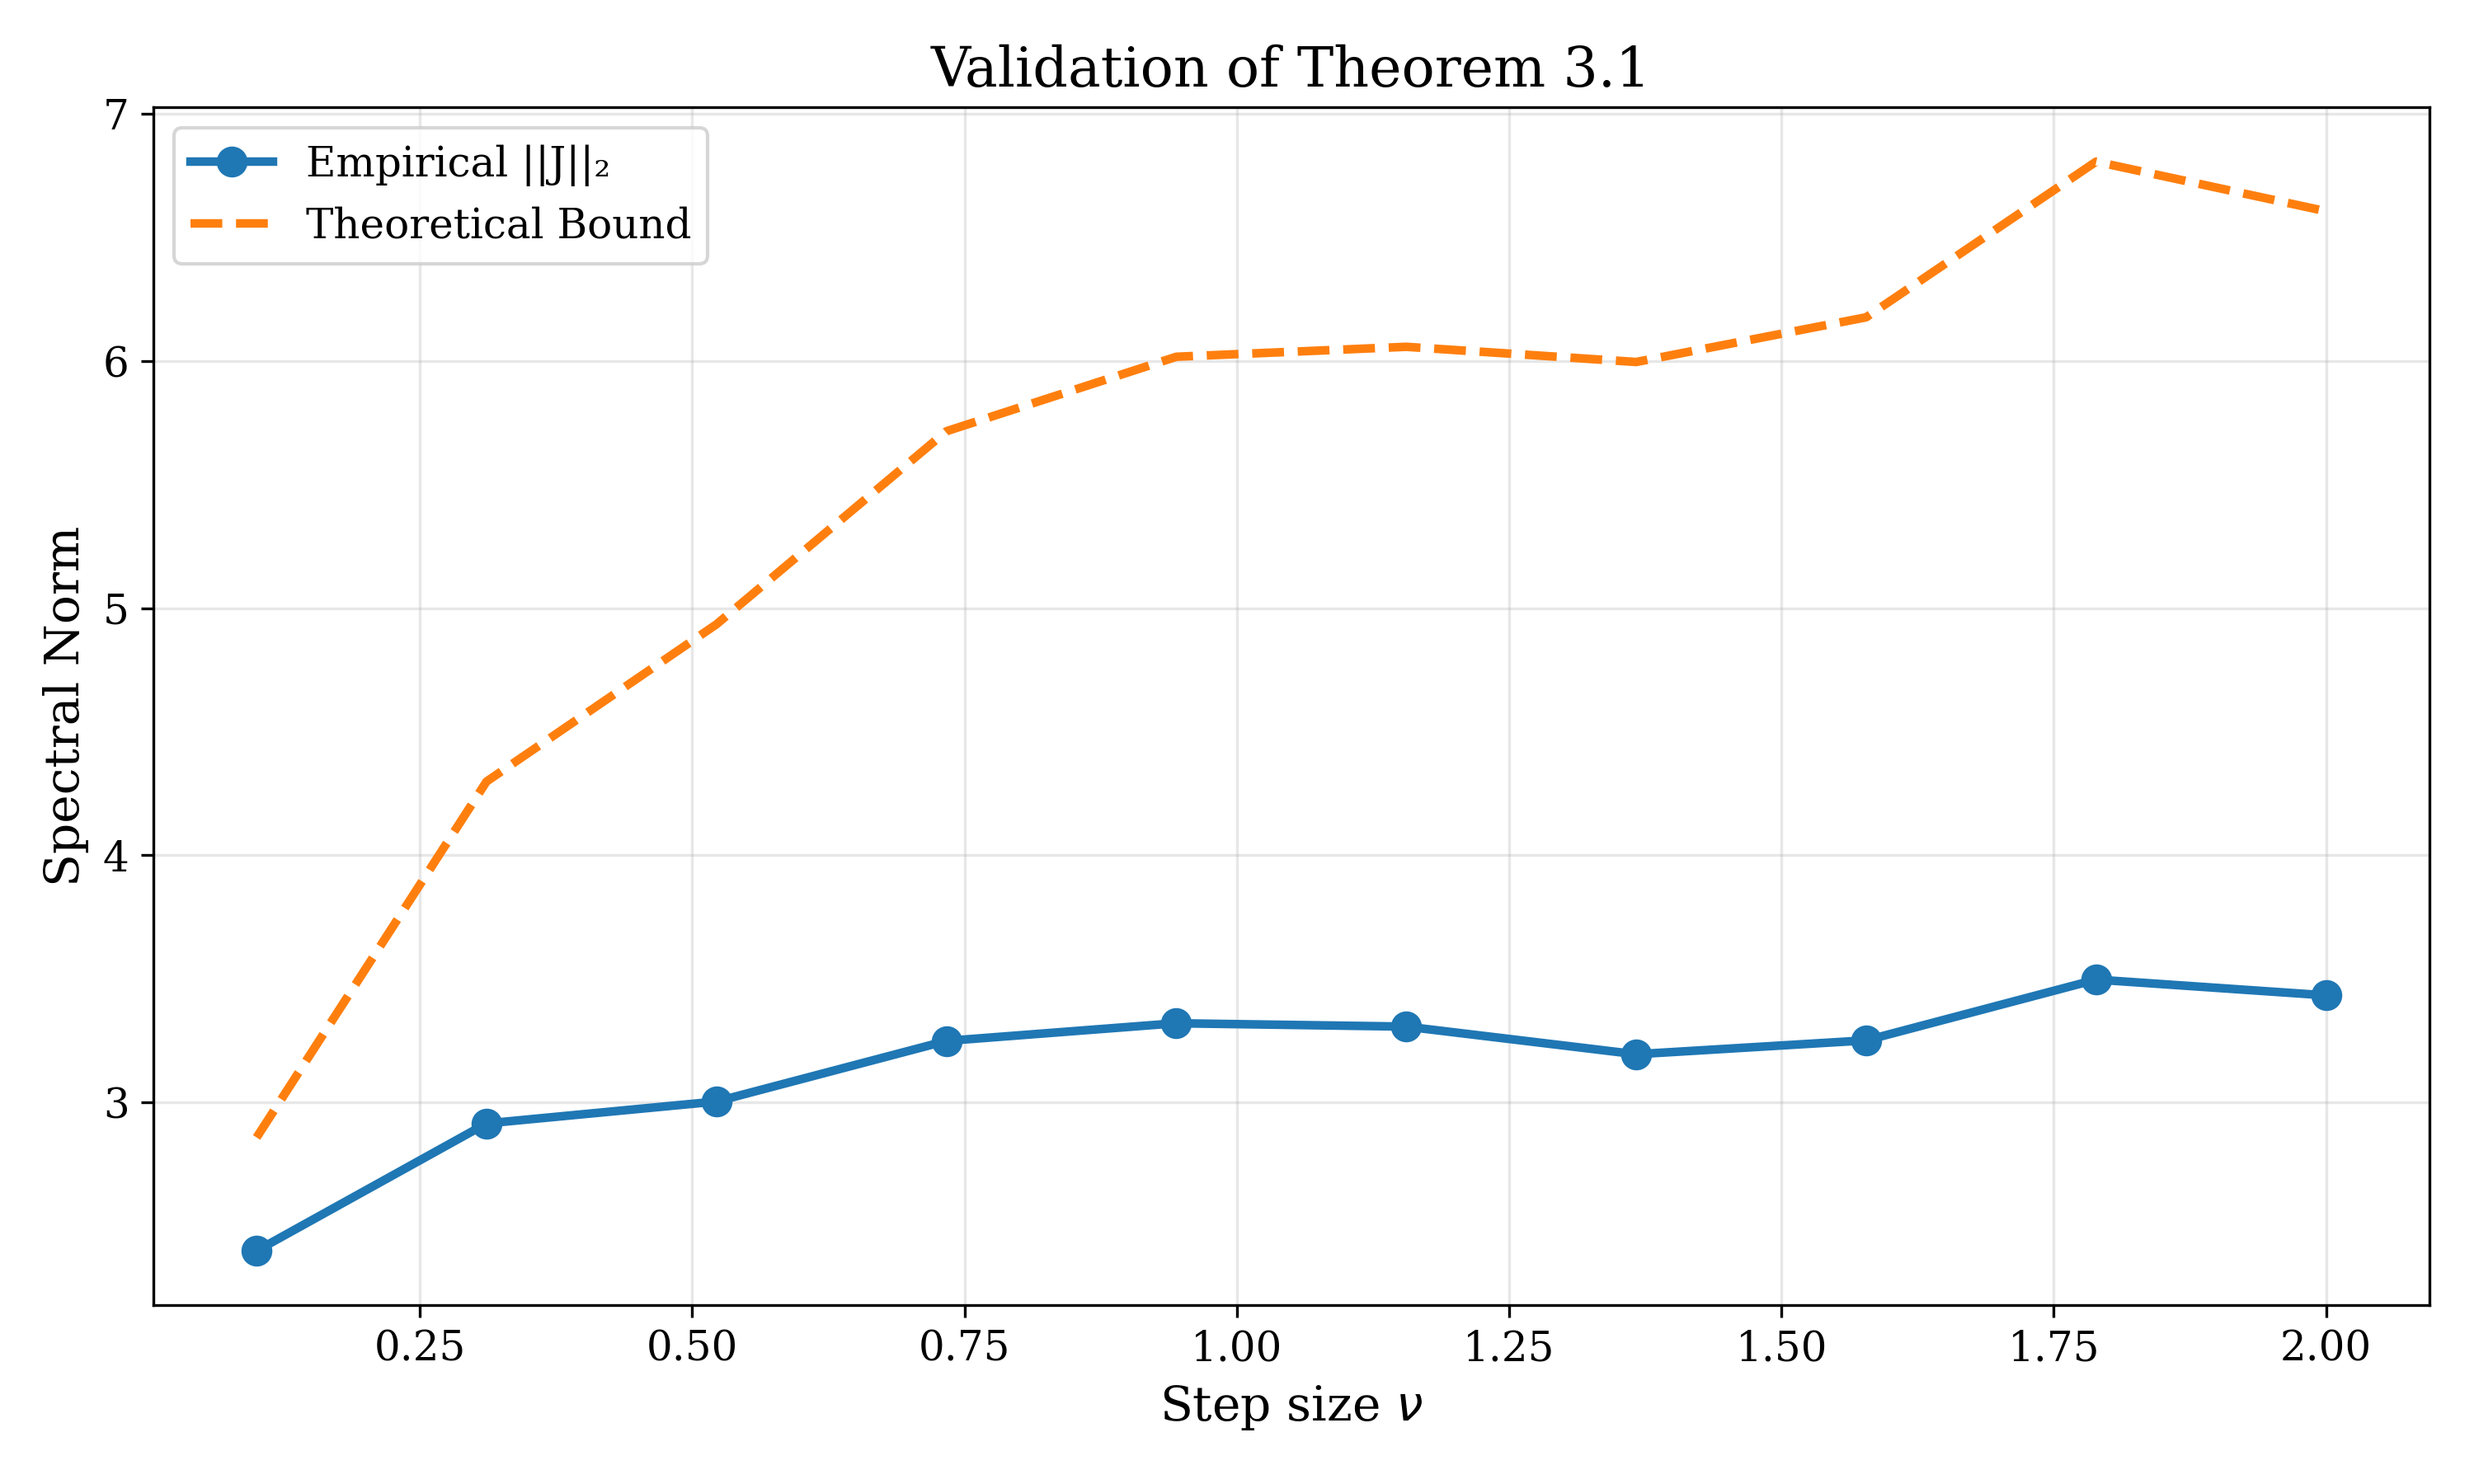
\includegraphics[width=\columnwidth]{fig1_bounds_validation.png}
    \caption{Validation of Theorem~\ref{thm:jacobian_bound_final}: The empirical Jacobian spectral norm (blue solid) versus the theoretical upper bound (orange dashed) as a function of the step coefficient $\nu$.}
    \label{fig:full_spectral}
\end{figure}

\subsection{Asymptotic Behavior: $O(1)$ Stability for Large $\nu$}
\label{ssec:exp_asymptotic}

Next, we validate the asymptotic compensation mechanism described in Theorem~\ref{thm:JF_asympt}. We sweep $\nu$ over two orders of magnitude ($0.1$ to $100$) using synthetic Gaussian inputs ($S=16$, $D=32$, $H=4$, $D_{ff}=64$).
Our theory predicts that as $\nu \to \infty$, the growth of row norms $r_U \sim \nu$ leads to an inverse scaling of the Jacobian $\gamma_{\max}/r_U \sim 1/\nu$, which cancels out the linear growth of the update term.

Figure~\ref{fig:asymptotic_synthetic} empirically confirms this prediction. The spectral norm grows sub-linearly for small $\nu$ and saturates at an $O(1)$ plateau for large $\nu$. This illustrates that RMS normalization provides a robust compensating mechanism that prevents unbounded gradient explosion even for very large implicit step sizes.

\begin{figure}[H]
    \centering
    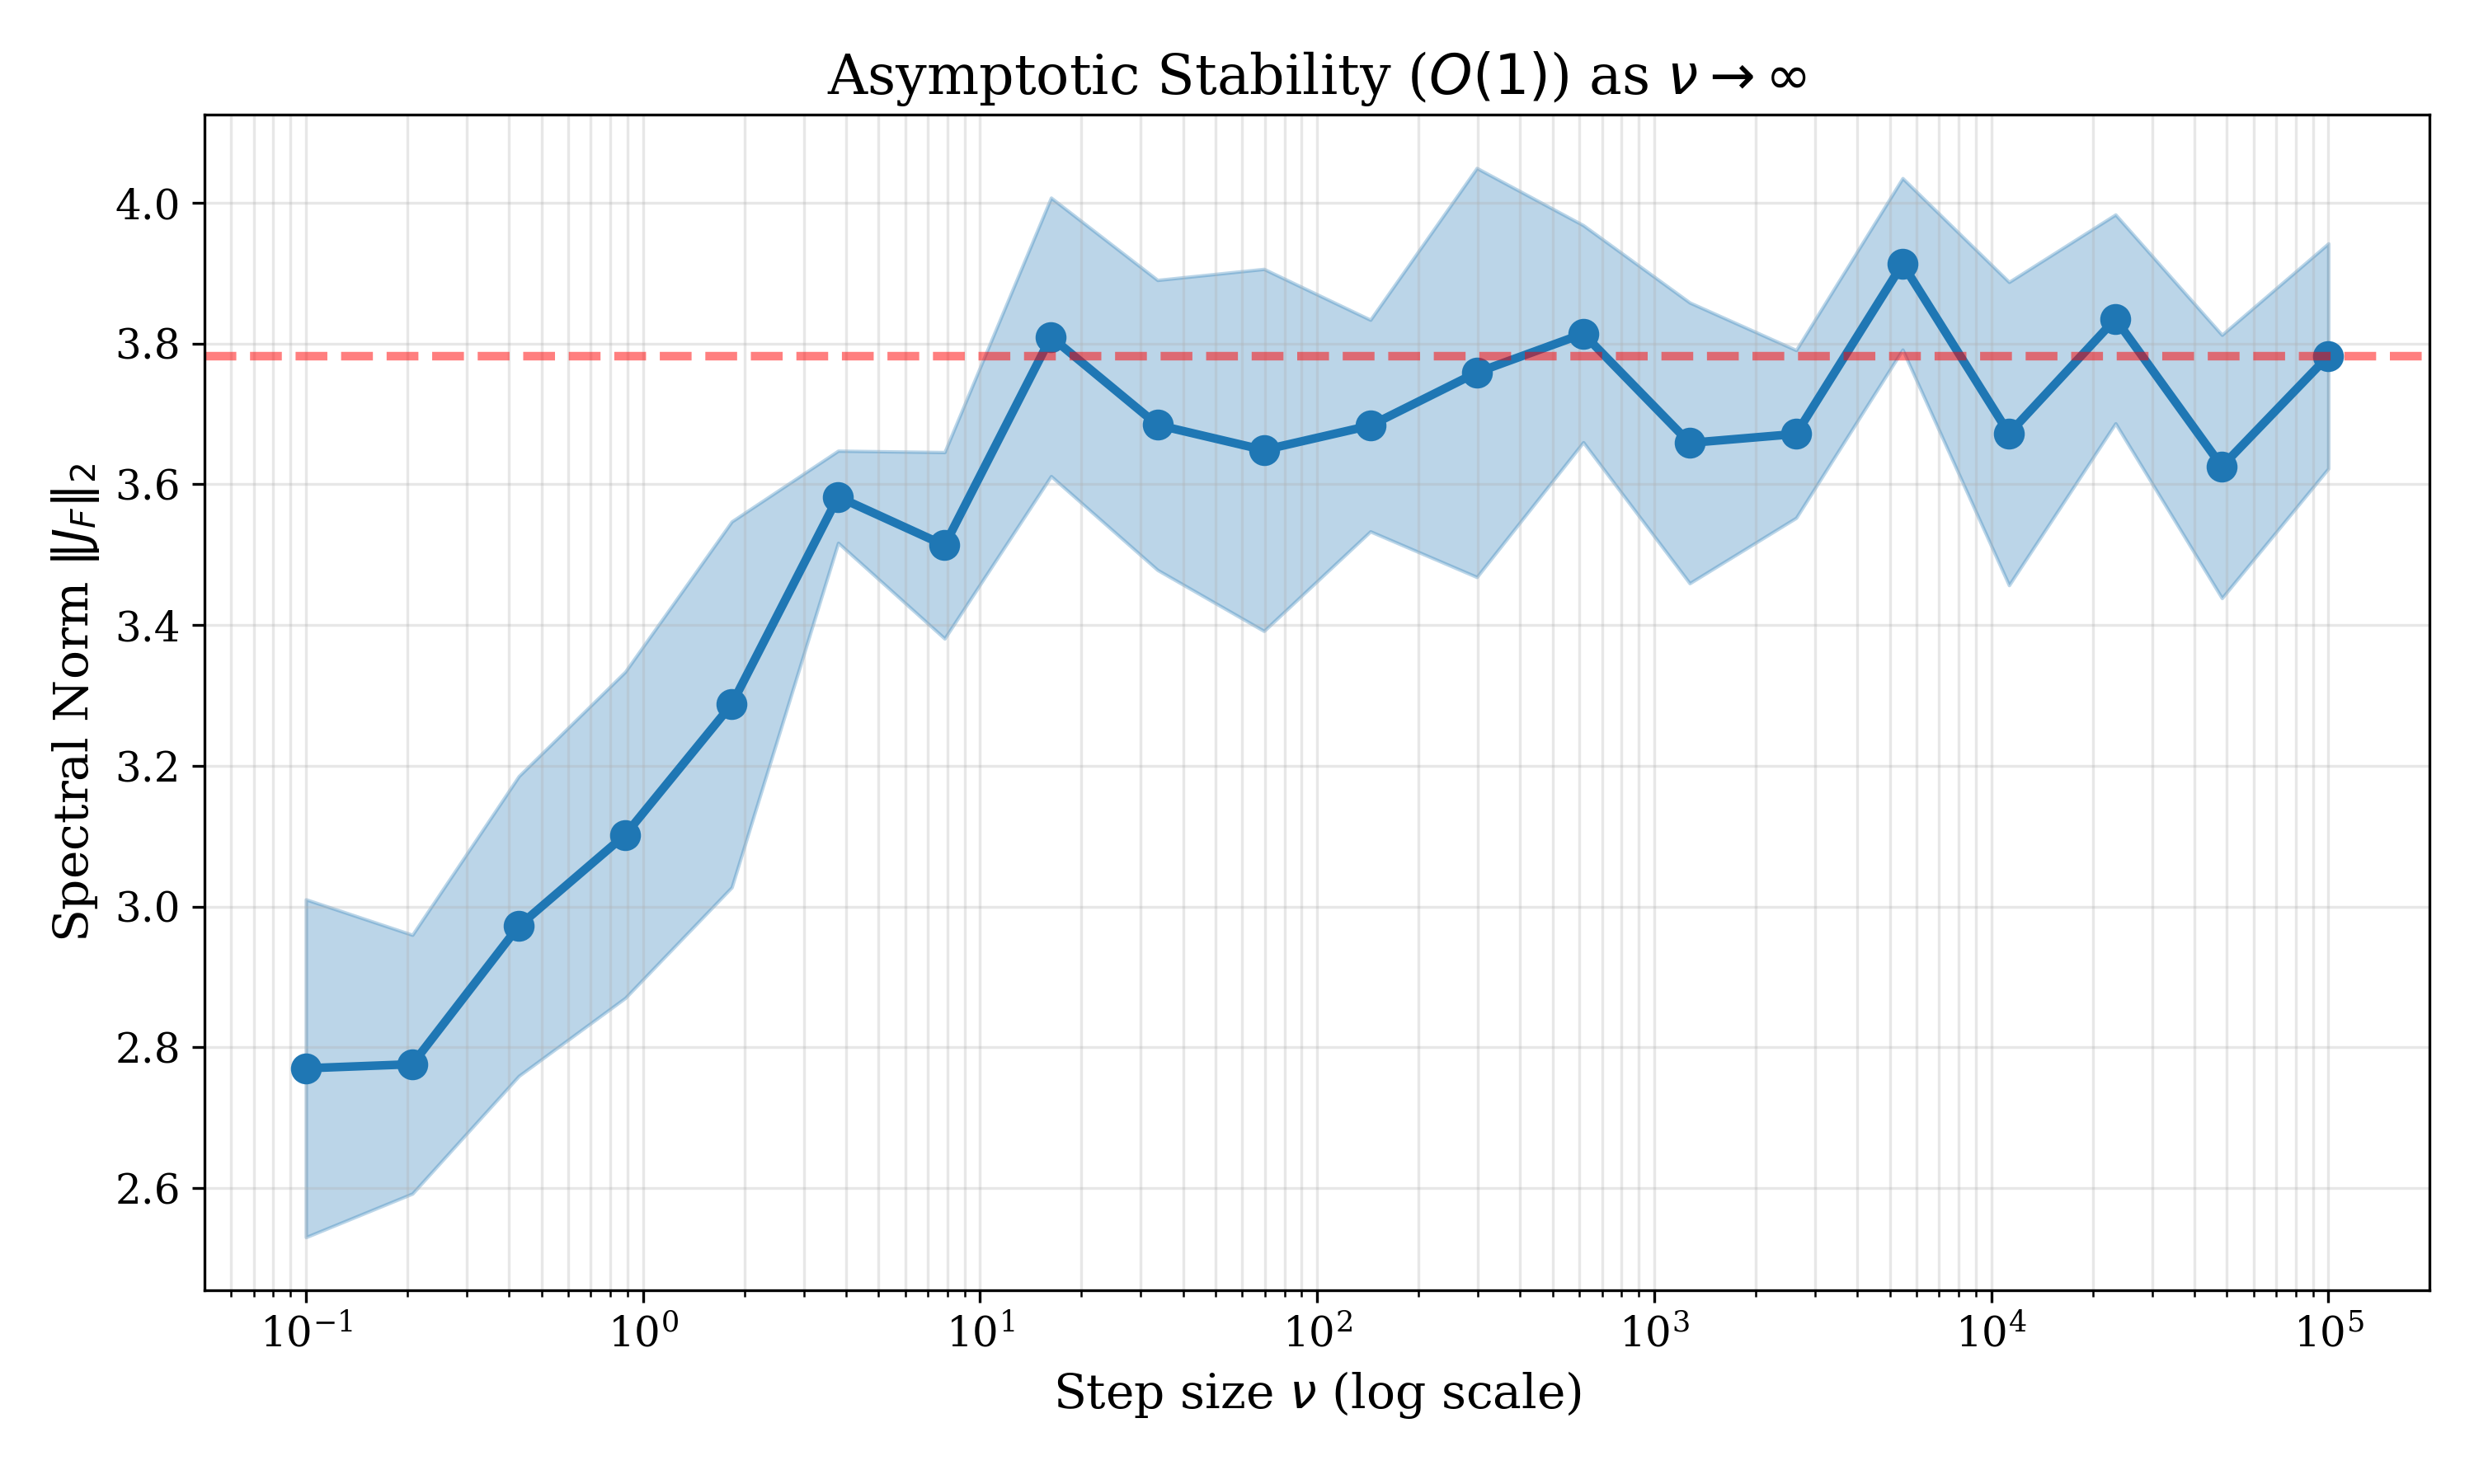
\includegraphics[width=\columnwidth]{fig2_asymptotic.png}
    \caption{Asymptotic stability as $\nu\to\infty$. The Jacobian spectral norm (log scale) converges to a constant value despite the increasing step size. The shaded region indicates the standard deviation over 10 random initializations.}
    \label{fig:asymptotic_synthetic}
\end{figure}

\subsection{Empirical Contraction Behaviour}
\label{ssec:exp_contraction}

While Jacobian analysis guarantees \textit{local} stability, we also check \textit{global} convergence by tracking $d_t = \|Y^{(t+1)} - Y^{(t)}\|_F$ over iterations on synthetic data ($X \sim \mathcal{N}(0,I)$) and CIFAR-10 embeddings.

% Figure~\ref{fig:lyapunov_comparison} demonstrates clear convergence in both settings: we observe rapid contraction on synthetic data as well as on CIFAR-10. In all cases $d_t \to 0$, and while increasing $\nu$ slows the contraction, it does not prevent it, indicating that RMSNorm contributes to robust global stability.

Figure~\ref{fig:lyapunov_comparison} demonstrates empirical convergence in both synthetic and CIFAR-10 settings. While Jacobian analysis primarily guarantees local stability, we observe rapid contraction of the state updates, indicating that the controlled Jacobian norm contributes to robust numerical behavior across iterations.

\begin{figure}[ht]
    \centering
 
        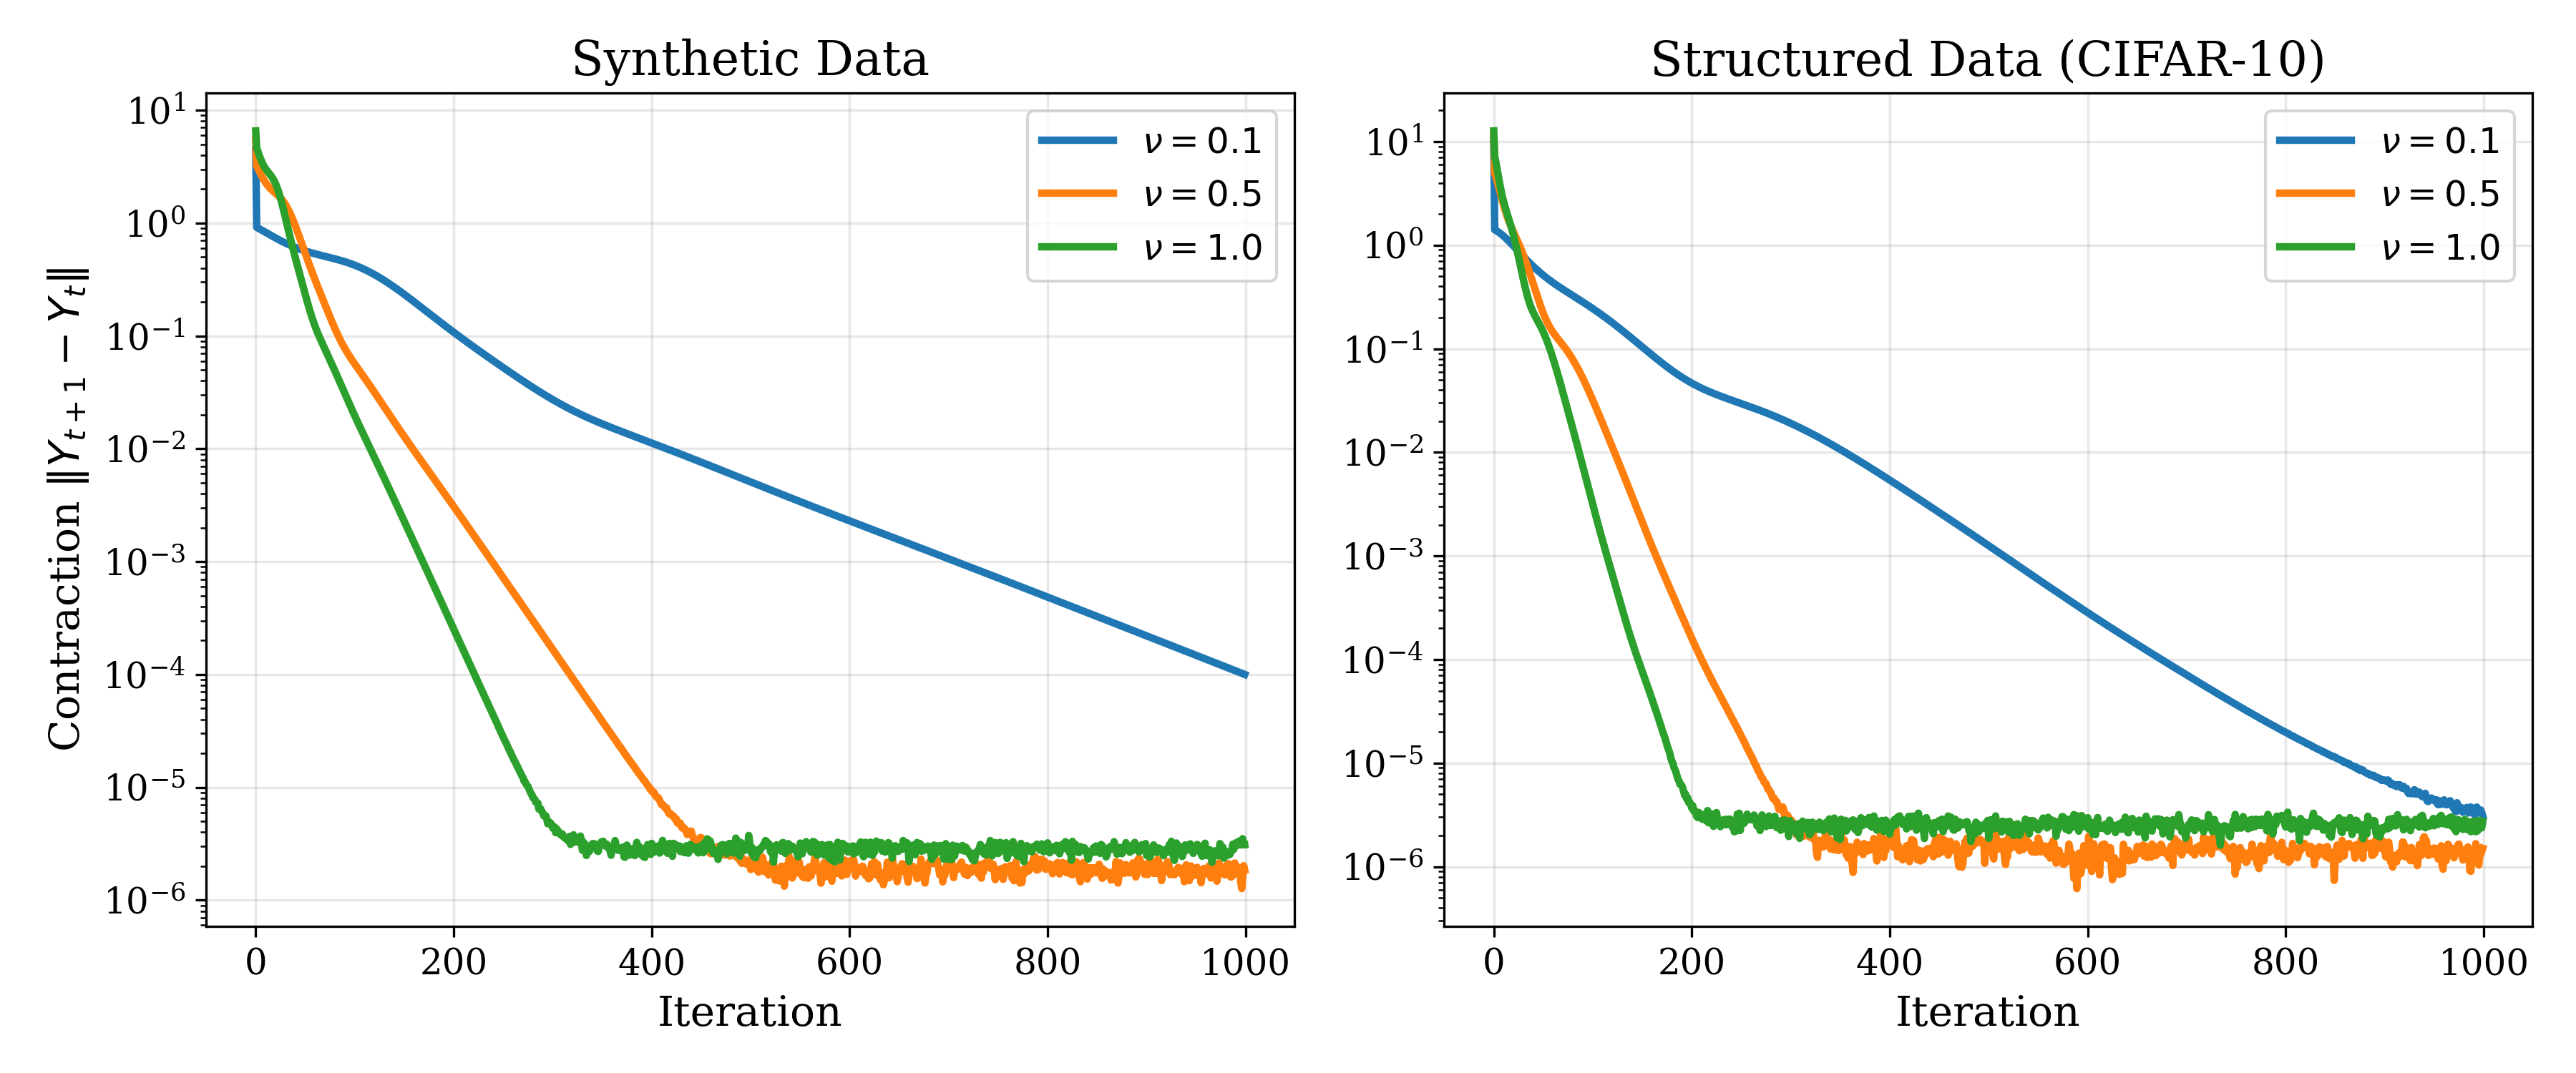
\includegraphics[width=\columnwidth]{fig3_contraction.png}
 
    \caption{Contraction dynamics on synthetic data (left) versus CIFAR-10 embeddings (right). The plots show the empirical convergence as the update magnitude $d_t$ diminishes over iterations.}
    \label{fig:lyapunov_comparison}
\end{figure}

\section{Conclusion}
We extended Jacobian-based stability analysis from SA-only blocks to full Transformer blocks with MSA and FFN. We derived an explicit upper bound on the full-block Jacobian spectral norm, showing that RMSNorm stabilizes this more complex setting. Experiments confirm that predicted stability matches empirical behavior. While conservative and relying on mild norm assumptions, our bounds demonstrate that Jacobian analysis is a robust tool for understanding looped Transformer dynamics and designing stable architectures.

While our analysis focuses on the Post-Norm architecture, the damping role of RMSNorm is expected to be universal. Future work could investigate Pre-Norm variants, where the normalization precedes the attention mechanism, potentially altering the sensitivity of the Jacobian to initialization.


% --- REFERENCES (Alphabetical order, Initials only) ---
\begin{thebibliography}{99}

\bibitem{agarwala2022deep}
A. Agarwala, S. S. Schoenholz, \emph{Deep equilibrium networks are sensitive to initialization statistics}, International Conference on Machine Learning, 2022, pp. 136--160.

\bibitem{bai2019deep}
S. Bai, J. Z. Kolter, V. Koltun, \emph{Deep equilibrium models}, Advances in Neural Information Processing Systems, 32, 2019.

\bibitem{bai2021stabilizing}
S. Bai, V. Koltun, J. Z. Kolter, \emph{Stabilizing equilibrium models by jacobian regularization}, arXiv preprint arXiv:2106.14342, 2021.

\bibitem{bal2023sequence}
M. Bal, A. Sengupta, \emph{Sequence Learning Using Equilibrium Propagation}, Thirty-Second International Joint Conference on Artificial Intelligence, 2023.

\bibitem{bansal2022end}
A. Bansal, et al., \emph{End-to-end algorithm synthesis with recurrent networks: Extrapolation without overthinking}, Advances in Neural Information Processing Systems, 35, 2022.

\bibitem{bietti2024birth}
A. Bietti, et al., \emph{Birth of a transformer: A memory viewpoint}, Advances in Neural Information Processing Systems, 36, 2024.

\bibitem{boedecker2012information}
J. Boedecker, et al., \emph{Information processing in echo state networks at the edge of chaos}, Theory in Biosciences, 131, 2012, pp. 205--213.

\bibitem{bruno2025emergence}
G. Bruno, F. Pasqualotto, A. Agazzi, \emph{Emergence of meta-stable clustering in mean-field transformer models}, International Conference on Learning Representations, 2025.

\bibitem{castin2023smooth}
V. Castin, P. Ablin, G. Peyr{\'e}, \emph{How Smooth Is Attention?}, International Conference on Machine Learning, 2024, pp. 5817--5840.

\bibitem{chang2019antisymmetricrnn}
B. Chang, et al., \emph{AntisymmetricRNN: A Dynamical System View on Recurrent Neural Networks}, International Conference on Learning Representations, 2019.

\bibitem{chowdhery2023palm}
A. Chowdhery, et al., \emph{Palm: Scaling language modeling with pathways}, Journal of Machine Learning Research, 24, 2023.

\bibitem{dehghani2018universal}
M. Dehghani, et al., \emph{Universal Transformers}, International Conference on Learning Representations, 2018.

\bibitem{erichson2021lipschitz}
N. B. Erichson, et al., \emph{Lipschitz Recurrent Neural Networks}, International Conference on Learning Representations, 2021.

\bibitem{geiping2025scaling}
J. Geiping, et al., \emph{Scaling up Test-Time Compute with Latent Reasoning: A Recurrent Depth Approach}, arXiv preprint arXiv:2502.05171, 2025.

\bibitem{geshkovski2023mathematical}
B. Geshkovski, et al., \emph{A mathematical perspective on transformers}, Bulletin of the American Mathematical Society, 62(3), 2025, pp. 427--479.

\bibitem{giannou2023looped}
A. Giannou, et al., \emph{Looped transformers as programmable computers}, International Conference on Machine Learning, 2023, pp. 11398--11442.

\bibitem{haber2017stable}
E. Haber, L. Ruthotto, \emph{Stable architectures for deep neural networks}, Inverse problems, 34(1), 2017.

\bibitem{hoover2024energy}
B. Hoover, et al., \emph{Energy transformer}, Advances in Neural Information Processing Systems, 36, 2023.

\bibitem{hopfield1982neural}
J. J. Hopfield, \emph{Neural networks and physical systems with emergent collective computational abilities}, PNAS, 79(8), 1982, pp. 2554--2558.

\bibitem{kajitsuka2023transformers}
T. Kajitsuka, I. Sato, \emph{Are Transformers with One Layer Self-Attention Using Low-Rank Weight Matrices Universal Approximators?}, International Conference on Learning Representations, 2024.

\bibitem{kingma2014adam}
D. P. Kingma, J. Ba, \emph{Adam: A method for stochastic optimization}, International Conference on Learning Representations, 2015.

\bibitem{krotov2021hierarchical}
D. Krotov, \emph{Hierarchical associative memory}, arXiv preprint arXiv:2107.06446, 2021.

\bibitem{lan2019albert}
Z. Lan, et al., \emph{ALBERT: A Lite BERT for Self-supervised Learning of Language Representations}, International Conference on Learning Representations, 2020.

\bibitem{lewandowski2024learning}
A. Lewandowski, et al., \emph{Learning Continually by Spectral Regularization}, International Conference on Learning Representations, 2025.

\bibitem{noci2022signal}
L. Noci, et al., \emph{Signal propagation in transformers: Theoretical perspectives and the role of rank collapse}, Advances in Neural Information Processing Systems, 35, 2022.

\bibitem{saunshi2025reasoning}
N. Saunshi, et al., \emph{Reasoning with latent thoughts: On the power of looped transformers}, arXiv preprint arXiv:2502.17416, 2025.

\bibitem{tomihari2025recurrent}
A. Tomihari, R. Karakida, \emph{Recurrent Self-Attention Dynamics: An Energy-Agnostic Perspective from Jacobians}, arXiv preprint arXiv:2505.19458, 2025.

\bibitem{vaswani2017attention}
A. Vaswani, et al., \emph{Attention is all you need}, CoRR, abs/1706.03762, 2017.

\bibitem{yang2022transformers}
Y. Yang, D. P. Wipf, et al., \emph{Transformers from an optimization perspective}, Advances in Neural Information Processing Systems, 35, 2022.

\bibitem{yoshida2017spectral}
Y. Yoshida, T. Miyato, \emph{Spectral norm regularization for improving the generalizability of deep learning}, arXiv preprint arXiv:1705.10941, 2017.

\bibitem{yun2019transformers}
C. Yun, et al., \emph{Are Transformers universal approximators of sequence-to-sequence functions?}, International Conference on Learning Representations, 2020.

\bibitem{zhang2019root}
B. Zhang, R. Sennrich, \emph{Root mean square layer normalization}, Advances in Neural Information Processing Systems, 32, 2019.

\end{thebibliography}



\newpage
\appendix
\section{Proofs}
\label{app:proofs}

\subsection{Proof of Theorem~\ref{thm:jacobian_bound_final}}
\label{app:jacobian-proof}
\begin{proof}

The proof strategy follows the framework established in~\cite{tomihari2025recurrentselfattentiondynamicsenergyagnostic}. We extend their analysis of the standalone self-attention layer to the full Transformer block by applying the chain rule to the composite structure including the FFN and multiple normalization layers.

First, recall the spectral norm bound for the Jacobian of the row-wise RMSNorm operation $f(u) = \RMS(u)$. Using Theorem A.3 from~\cite{tomihari2025recurrentselfattentiondynamicsenergyagnostic} (and as derived in our Lemma logic), we have:
\begin{equation}
    \norm{\frac{\partial \RMS(u)}{\partial u}}_2 \le \frac{\gamma_{\max}}{\norm{u}_2}.
\end{equation}

Now consider the full iterative update $F(Y)=\RMS(U)$ where $U = Y + \nu(C + \TB(Y))$.  
By the chain rule and the lower bound $\norm{U_{[i,:]}} \ge r_U$:
\begin{align}
    \norm{J_F(Y)}_2 
    &\le \frac{\gamma_{\max}}{r_U} \norm{I + \nu J_{\TB}(Y)}_2 \\
    &\le \frac{\gamma_{\max}}{r_U} (1 + \nu \norm{J_{\TB}(Y)}_2).
\end{align}

Next, we evaluate $\norm{J_{\TB}(Y)}_2$. Recall the sequential Post-Norm structure:

1. $Y' = \RMS(Z_1)$ where $Z_1 = Y + \MSA(Y)$.
    
2. $\TB(Y) = \RMS(Z_2)$ where $Z_2 = Y' + \FFN(Y')$.

Applying the chain rule to the second sub-block (FFN):
\begin{align}
    \norm{\frac{\partial \TB}{\partial Y'}}_2 
    &\le \frac{\gamma_{\max}}{r_{out}} \norm{I + J_{\FFN}(Y')}_2 \\
    &\le \frac{\gamma_{\max}}{r_{out}} (1 + \norm{J_{\FFN}}).
\end{align}
Applying the chain rule to the first sub-block (MSA):
\begin{align}
    \norm{\frac{\partial Y'}{\partial Y}}_2 
    &\le \frac{\gamma_{\max}}{r_{in}} \norm{I + J_{\MSA}(Y)}_2 \\
    &\le \frac{\gamma_{\max}}{r_{in}} (1 + \norm{J_{\MSA}}).
\end{align}

Finally, combining these via the chain rule $J_{\TB}(Y) = \frac{\partial \TB}{\partial Y'} \frac{\partial Y'}{\partial Y}$:
\begin{multline}
\norm{J_{\TB}(Y)}_2 
\le \left( \frac{\gamma_{\max}}{r_{out}} 
       \big(1 + \norm{J_{\FFN}}\big) \right) \\
       \times \left( \frac{\gamma_{\max}}{r_{in}}
       \big(1 + \norm{J_{\MSA}}\big) \right) =\\
= \frac{\gamma_{\max}^2}{r_{out} r_{in}} 
   \big(1 + \norm{J_{\FFN}}\big) 
   \big(1 + \norm{J_{\MSA}}\big).
\end{multline}

Substituting this back into the expression for $\norm{J_F(Y)}_2$ yields the theorem statement.
\end{proof}

\subsection{Proof of Theorem~\ref{thm:JF_asympt}}
\label{app:JF_asympt}
\begin{proof}
Our derivation adapts the asymptotic argument from~\cite{tomihari2025recurrentselfattentiondynamicsenergyagnostic} to the full block setting. Specifically, we utilize the same projection-based decomposition of the RMSNorm Jacobian to demonstrate the scaling behavior.

Define, for each $i$, the projection
\begin{align}
P_i \coloneqq I_D - \frac{Y_{[i,:]}Y_{[i,:]}^{\top}}{\|Y_{[i,:]}\|_{2}^2},
\end{align}
so that $\| P_i\|_{2} = 1$.  
Let $D_{\gamma} \coloneqq \operatorname{diag}(\gamma)$, and define the block factors
\begin{align}
A_i(\nu) \coloneqq \frac{1}{\| U_{[i,:]} \|_{2}}\,D_{\gamma}\,P_i,
\\
A(\nu) \coloneqq \operatorname{blockdiag}\left(\{A_i(\nu)\}_{i=1}^S\right).
\end{align}
Note that $U = Y + \nu \Delta Y$. By the triangle inequality, for each $i$,
\begin{align}
\| Y_{[i,:]}+\nu\,\Delta Y_{[i,:]} \|_{2}
\;\ge\; \nu\,\| \Delta Y_{[i,:]}\|_{2} - \| Y_{[i,:]}\|_{2}.
\end{align}

Recall that $Y$ is the output of the previous layer (normalization), so that $\|Y_{[i,:]}\|_{2} \leq \gamma_{\max}$ (bounded by scale parameters).

Assume the non-degeneracy condition $\min_i \|\Delta Y_{[i,:]}\|_{2} \ge \varepsilon > 0$.  
Then, for a sufficiently large $\nu$, specifically $\nu \ge 2\gamma_{\max} /\varepsilon$, we have:
\begin{align}
\| Y_{[i,:]}+\nu\,\Delta Y_{[i,:]} \|_{2}
&\ge  \nu\,\|\Delta Y_{[i,:]} \|_{2} - \|Y_{[i,:]}\|_{2} \\
&\ge \frac{\nu}{2}\,\|\Delta Y_{[i,:]}\|_{2}.
\end{align}

Using submultiplicativity and $\|P_i\|_{2}=1$, we obtain for the normalization Jacobian block $J_{\RMS}$:
\begin{align}
\| A_i(\nu) \|_{2}
&= \frac{\| D_{\gamma}\,P_i\|_{2}}{\| Y_{[i,:]}+\nu\,\Delta Y_{[i,:]} \|_{2}} \\
&\le \frac{\gamma_{\max}}{\frac{\nu}{2} \|\Delta Y_{[i,:]}\|_{2}} \\
&\le \frac{2\gamma_{\max}}{\nu \varepsilon}.
\end{align}

For a block-diagonal matrix, the operator norm equals the maximum block norm; thus $\| A(\nu) \|_{2} \le \frac{2\gamma_{\max}}{\nu \varepsilon}$.

The full Jacobian is (by chain rule):
\begin{align}
J_F(Y) = A(\nu) \cdot (I + \nu J_{\TB}(Y)).
\end{align}
Taking the norm:
\begin{align}
\|J_F(Y)\|_2 
&\le \|A(\nu)\|_2 (1 + \nu \|J_{\TB}(Y)\|_2) \\
&\le \frac{2\gamma_{\max}}{\nu \varepsilon} (1 + \nu K) \\
&= \frac{2\gamma_{\max}}{\nu \varepsilon} + \frac{2\gamma_{\max} K}{\varepsilon},
\end{align}
where $K$ is the bound on $\|J_{\TB}\|$ from Theorem~\ref{thm:jacobian_bound_final}, which does not depend on $\nu$.
Taking the limit $\nu \to \infty$, the first term vanishes and the second term is constant. Thus:
\begin{align}
\|J_F(Y)\|_2 = O(1).
\end{align}
\end{proof}

\newpage

Дмитрий Василенко, Илья Степанов, Вадим Касюк, Глеб Карпеев, Андреей Грабовой. Якобиан-анализ рекуррентного блока трансформера

\begin{abstract}
Рекуррентные трансформеры представляют собой эффективный подход к моделированию глубоких вычислений, однако их использование в итерационных сценариях требует стабильной динамики. В работе исследуется динамика якобиана полного блока трансформера, включающего многоголовое внимание (MSA), сети прямого распространения (FFN) и RMS-нормализацию. Выведена верхняя граница спектральной нормы якобиана и показана роль RMS-нормализации в предотвращении взрыва градиентов.
\end{abstract}

\keywords{рекуррентные трансформеры, динамика якобиана, RMS-нормализация, анализ стабильности.}

\end{document}